\subsection{Omni Rollup}

The Omni Rollup is a robust framework designed to facilitate cross-chain transactions across multiple Layer 1 (L1) blockchains within the Omnichain ecosystem. It deploys smart contracts on L1 chains that support them, managing transaction validation, state updates, and communication with the rollup. For L1 chains that do not support smart contracts, Omni Rollup uses direct addresses (vaults) to handle asset custody and processing. Execution within the rollup can be configured in two ways: a shared executor maintaining isolated states for each supported chain, ensuring resource optimization and centralized logic, or separate executors for each chain, which provide high isolation and allow chain-specific customizations.  

At the core of its operation is the Omni Sequencer, a shared transaction coordinator responsible for organizing and ordering transactions. The sequencer collects transactions from various mempools and solvers, bundles them into batches, and determines a global order. A commitment for this order is created by hashing the ordered list of transaction bundles, producing a cryptographic digest that is published on a Data Availability (DA) layer. This commitment ensures that all participants can verify the integrity of the transaction order without accessing all transaction data. Each bundled transaction follows a specific format, comprising the source and destination chain IDs, the transaction payload, a timestamp, and a unique nonce to prevent replay attacks.  

Once the order is committed, the Omni Sequencer distributes the bundled transactions to the respective rollups for block creation. Each rollup verifies the transaction order against the commitment on the DA layer and uses the Prover network to validate state transitions. The Prover Network generates zero-knowledge (zk) proofs to confirm state correctness and prevent fraudulent updates. The rollup then updates the state of its respective chain and sends the updated state along with the zk proof to the L1 chain for final inclusion in its block. For non-contract-based chains, the proof will be sent to a client for verification. 
\begin{figure}[h!]
    \centering
    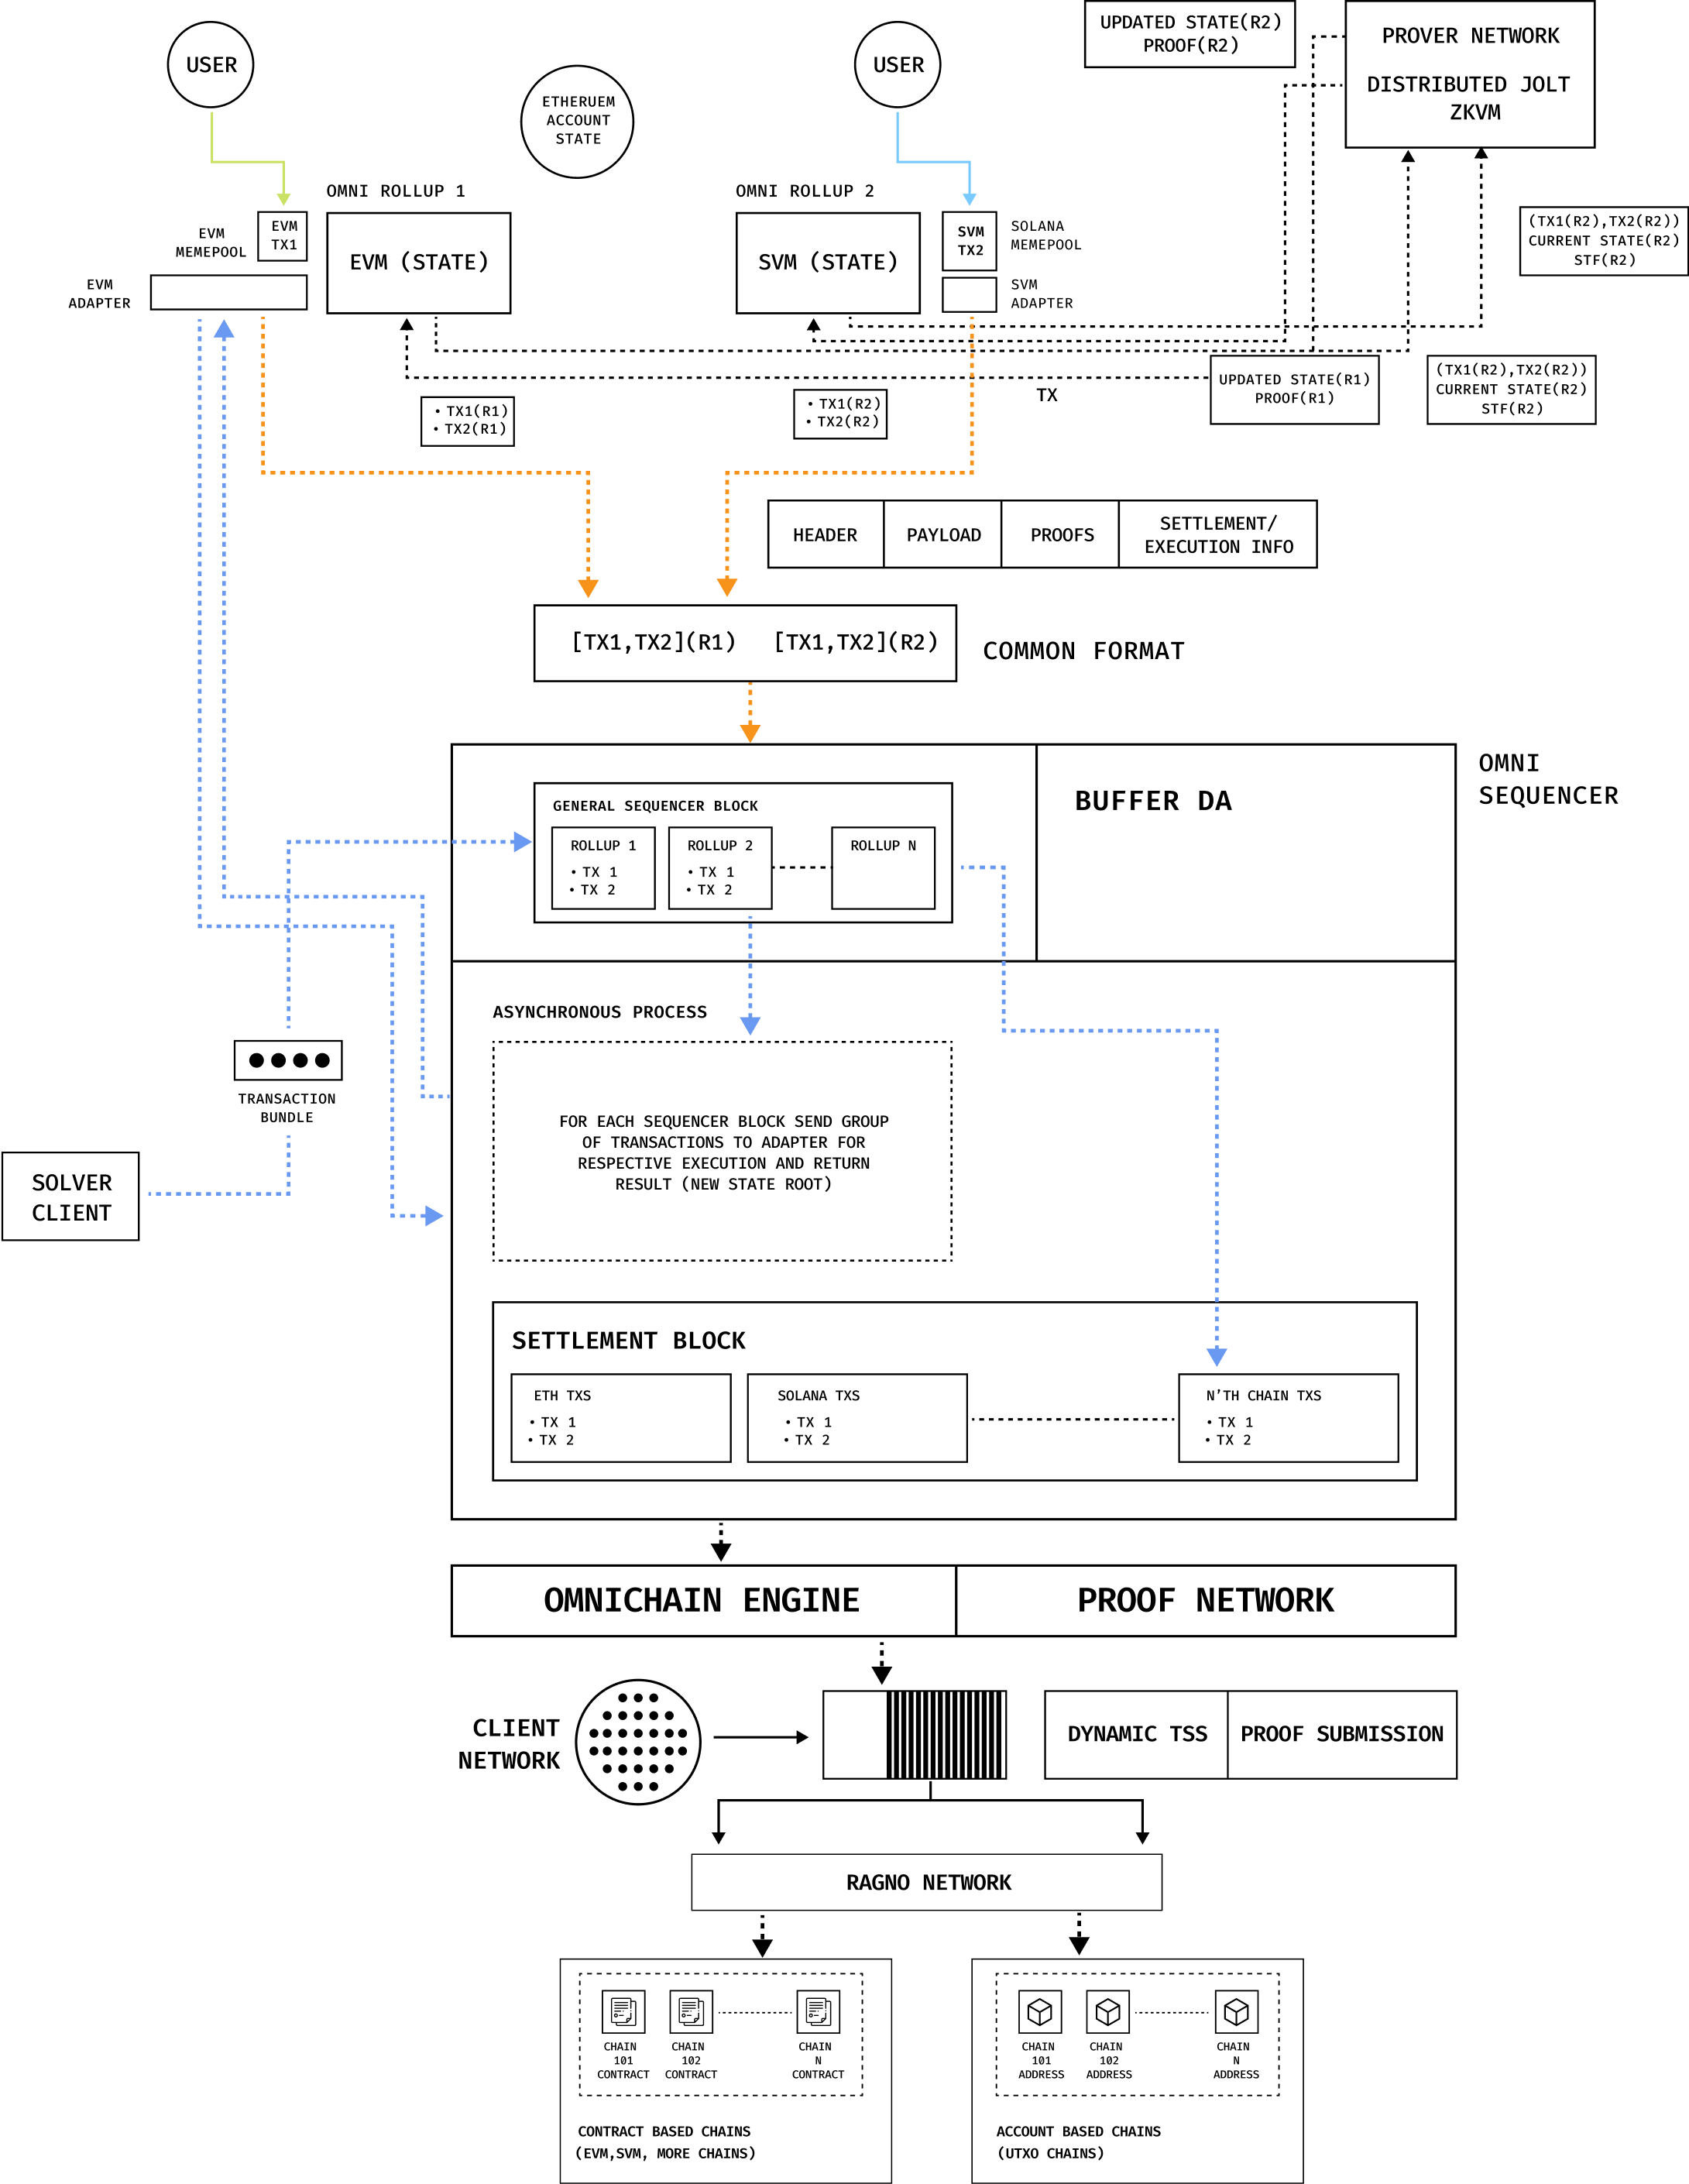
\includegraphics[width=0.99\linewidth]{figure/rollup.png}
    \caption{Omni Rollup Illustration}
    \label{fig:rollup}
\end{figure}
This architecture ensures scalability by efficiently bundling and ordering transactions, security through zk proofs and commitments, and interoperability by supporting both contract-enabled and other chains. The flexible executor configurations enable adaptation to diverse performance and isolation needs, making the Omni Rollup a critical component of the Omnichain web for seamless cross-chain transaction processing.



\subsubsection{Linera Microchains}

Linera~\cite{linera} introduces an innovative blockchain architecture centered around microchains, which are lightweight chains operating in parallel within a shared set of validators. This design separates the roles of block proposal and validation, often delegating block production to users themselves. Such an approach allows for an unlimited number of microchains to run concurrently, ensuring low transaction fees, rapid finality, and direct user access to on-chain data.

Linera’s core innovation lies in its microchain model, which is designed to scale Web3 applications predictably while taking advantage of modern cloud infrastructure. Key aspects include:
\begin{itemize}
    \item Elastic Validators: Validators function as scalable Web2-like services that validate and execute transactions across many microchains in parallel.
    
    \item User-Owned Microchains: Users own and maintain their own microchains, separating block production from validation.

    \item Integrated Multi-Chain Approach: Each validator manages all microchains, enabling asynchronous cross-chain messaging and parallel execution.

    \item Cross-Chain Messaging: Validators manage internal network communication between microchains to enable interoperability.

    \item Low-Latency Block Submission: Users submit blocks directly to validators without relying on a mempool, ensuring fast processing.

    \item Validator Independence: Validators do not interact with each other except for public chains owned by Linera’s infrastructure. Synchronization is handled by chain owners, and inactive chains impose no computational cost beyond storage.
\end{itemize}

Every validator maintains a map containing the states of all microchains, indexed by their identifiers. Clients track the state of only a subset of relevant chains, acting as full nodes only for those chains. This ensures efficient state management and reduces the computational burden on users.
Linera supports a theoretically unlimited number of microchains, allowing Web3 applications to maintain predictable performance at scale.

In conclusion,Linera’s microchain-based architecture provides a scalable, efficient, and user-friendly solution to traditional blockchain limitations. By decoupling block production from validation and leveraging elastic validators, Linera achieves the performance necessary for large-scale decentralized applications while maintaining decentralization and efficiency.



\subsubsection{Different Types of Rollups}
We are considering all different possibilities for cross-chain rollups. Along with omni-rollup, we are going to support existing and any private rollup as well with our cross-chain ecosystem. 

\begin{itemize}
    \item \textbf{Omni Rollup with Shared Executor}
    
    This architecture leverages a shared executor to oversee the states of all supported chains within a unified framework. The shared executor ensures efficient processing of cross-chain transactions while maintaining isolated state management for each chain, preventing conflicts, and preserving chain-specific integrity. This design simplifies interchain communication, but it necessitates robust mechanisms to mitigate state interference and establish trust in the shared execution layer. It is particularly well-suited for streamlined cross-chain dApps that benefit from a unified transaction coordinator.

 \begin{figure}[h!]
    \centering
    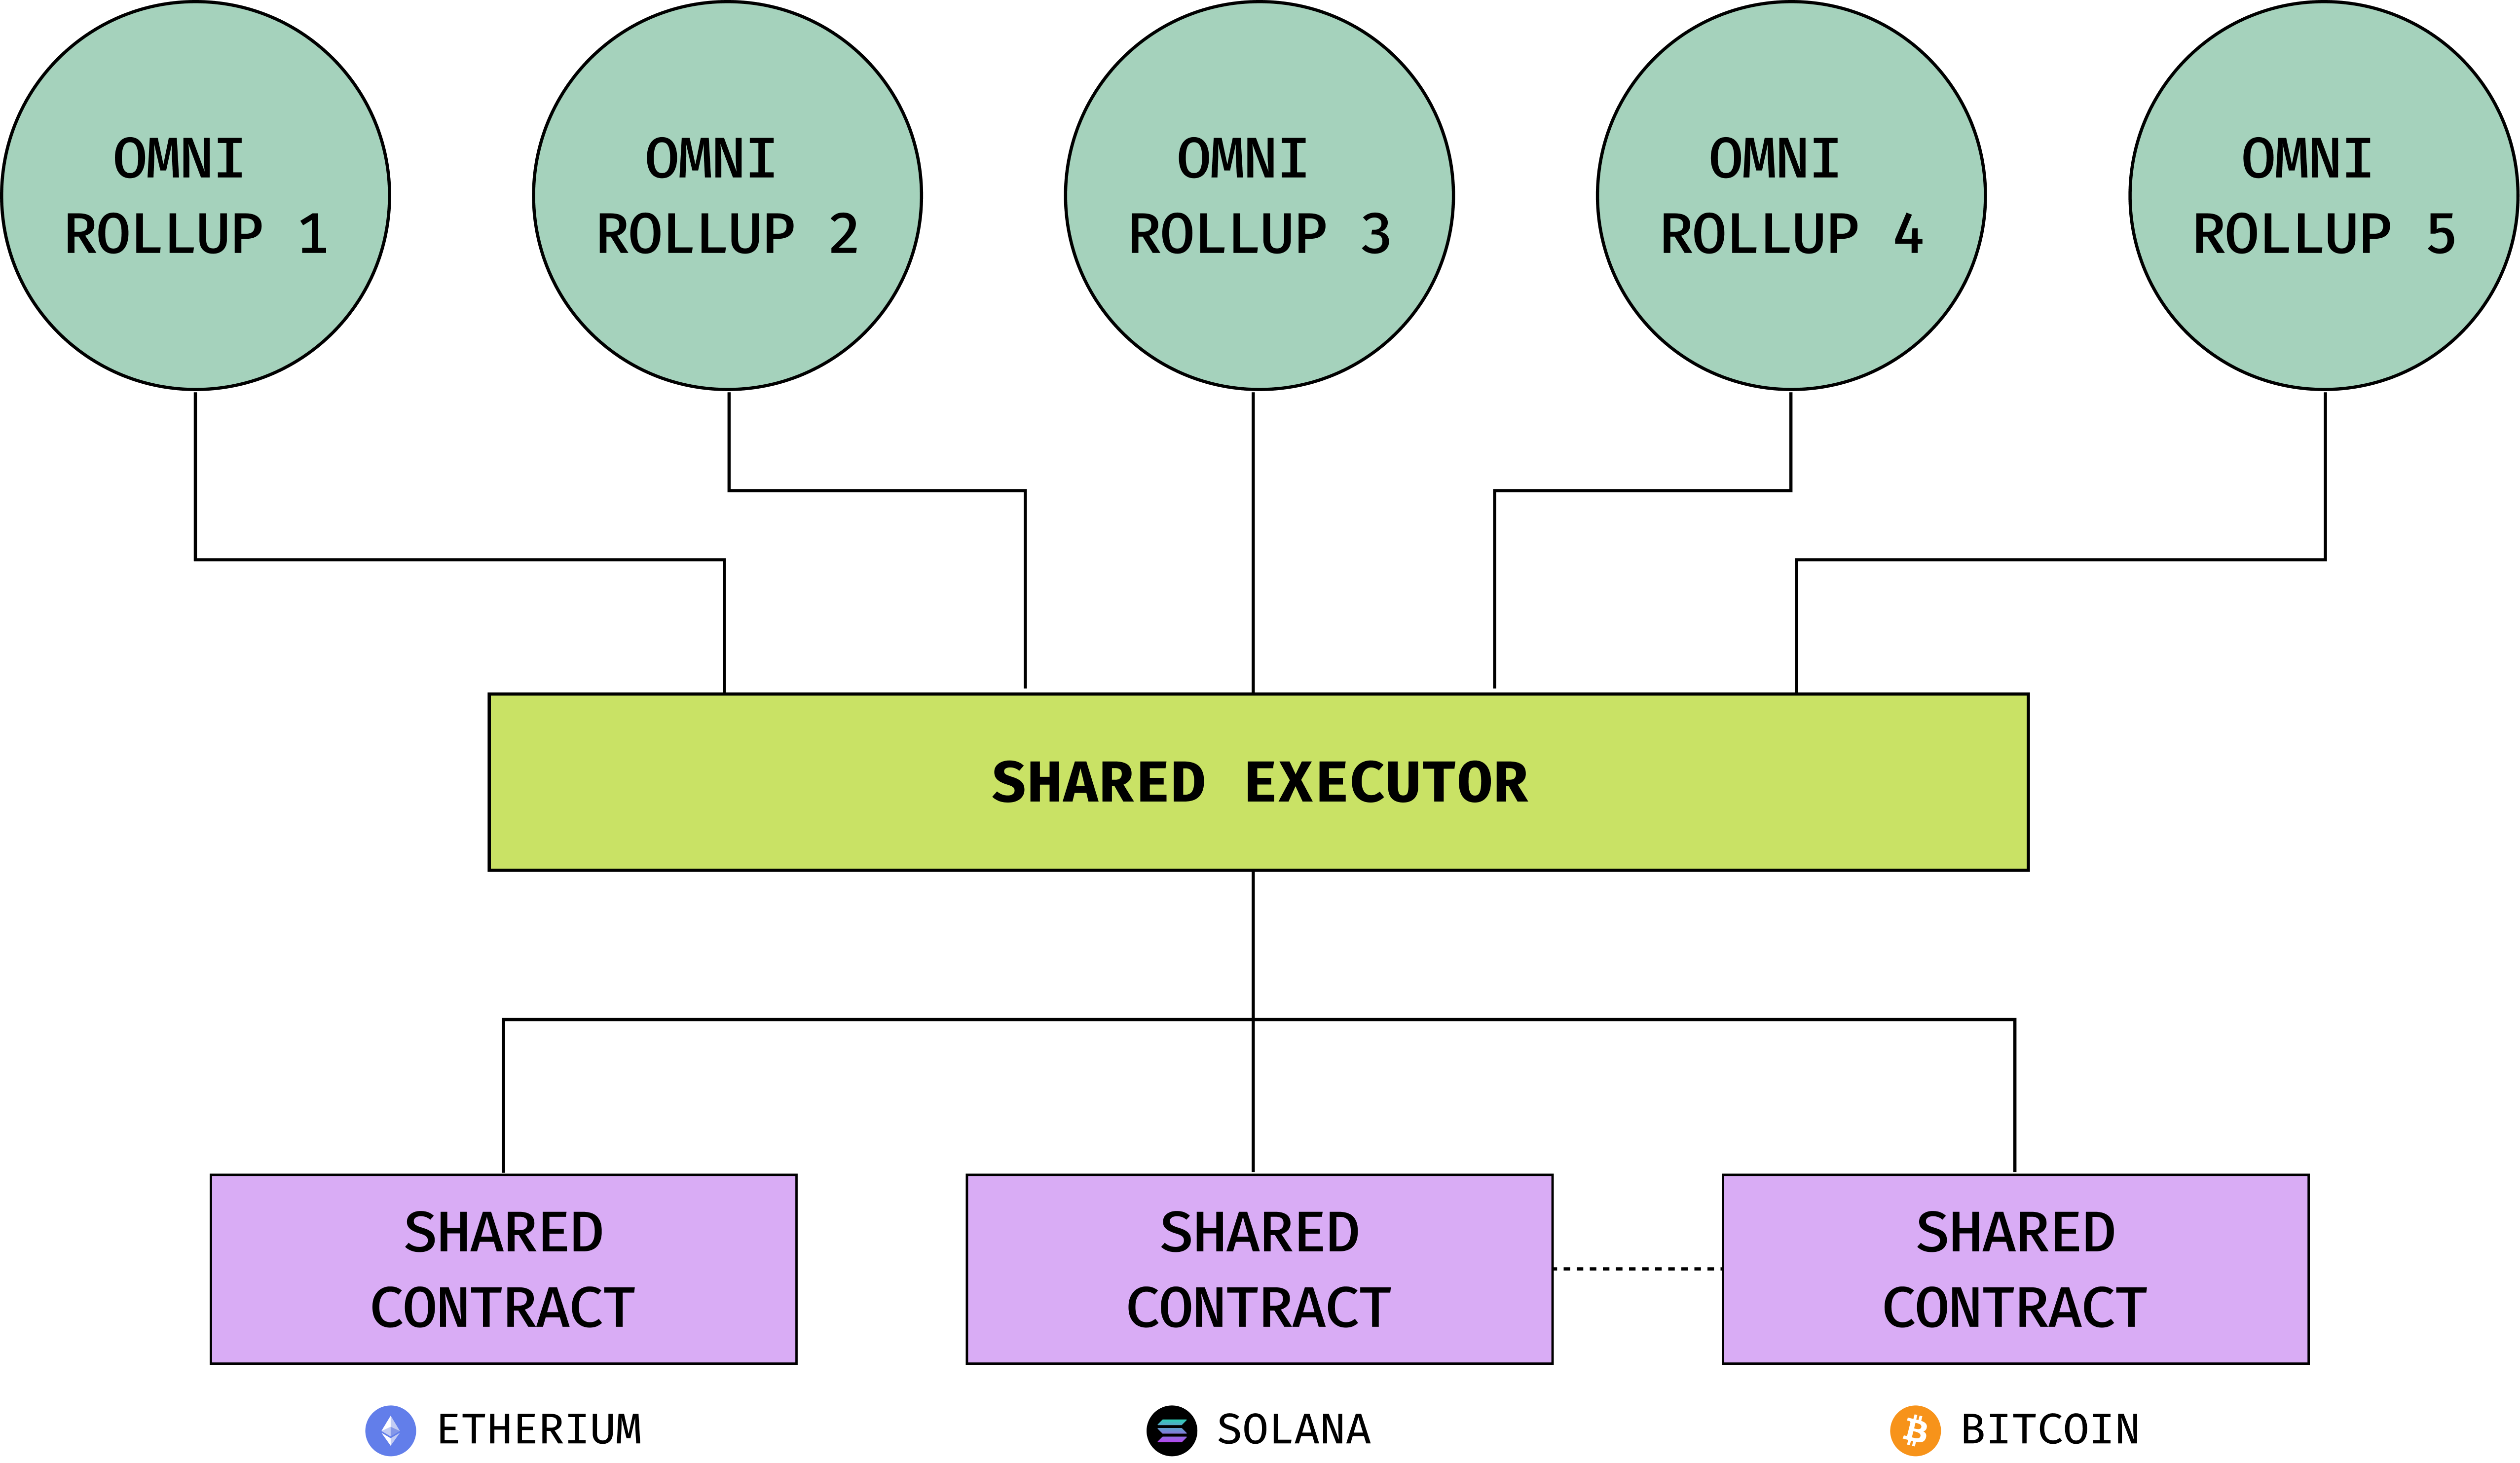
\includegraphics[width=0.9\linewidth]{figure/shared.png}
    \caption{Omni Rollup With Shared Executor}
    \label{fig:shared_rollup}
\end{figure}


    \item \textbf{Omni Rollup with Dedicated Executors for Each Chain}  

    In this setup, each supported chain operates with its own dedicated execution layer, ensuring autonomous state management while remaining part of the broader omnichain framework. This modular architecture improves resilience and scalability by isolating execution responsibilities per chain. However, advanced protocols are required for interoperability to ensure seamless cross-chain consistency and coordination. This approach is ideal for applications that require independent chain control in conjunction with flexible and efficient cross-chain interactions.
 \begin{figure}[h!]
    \centering
    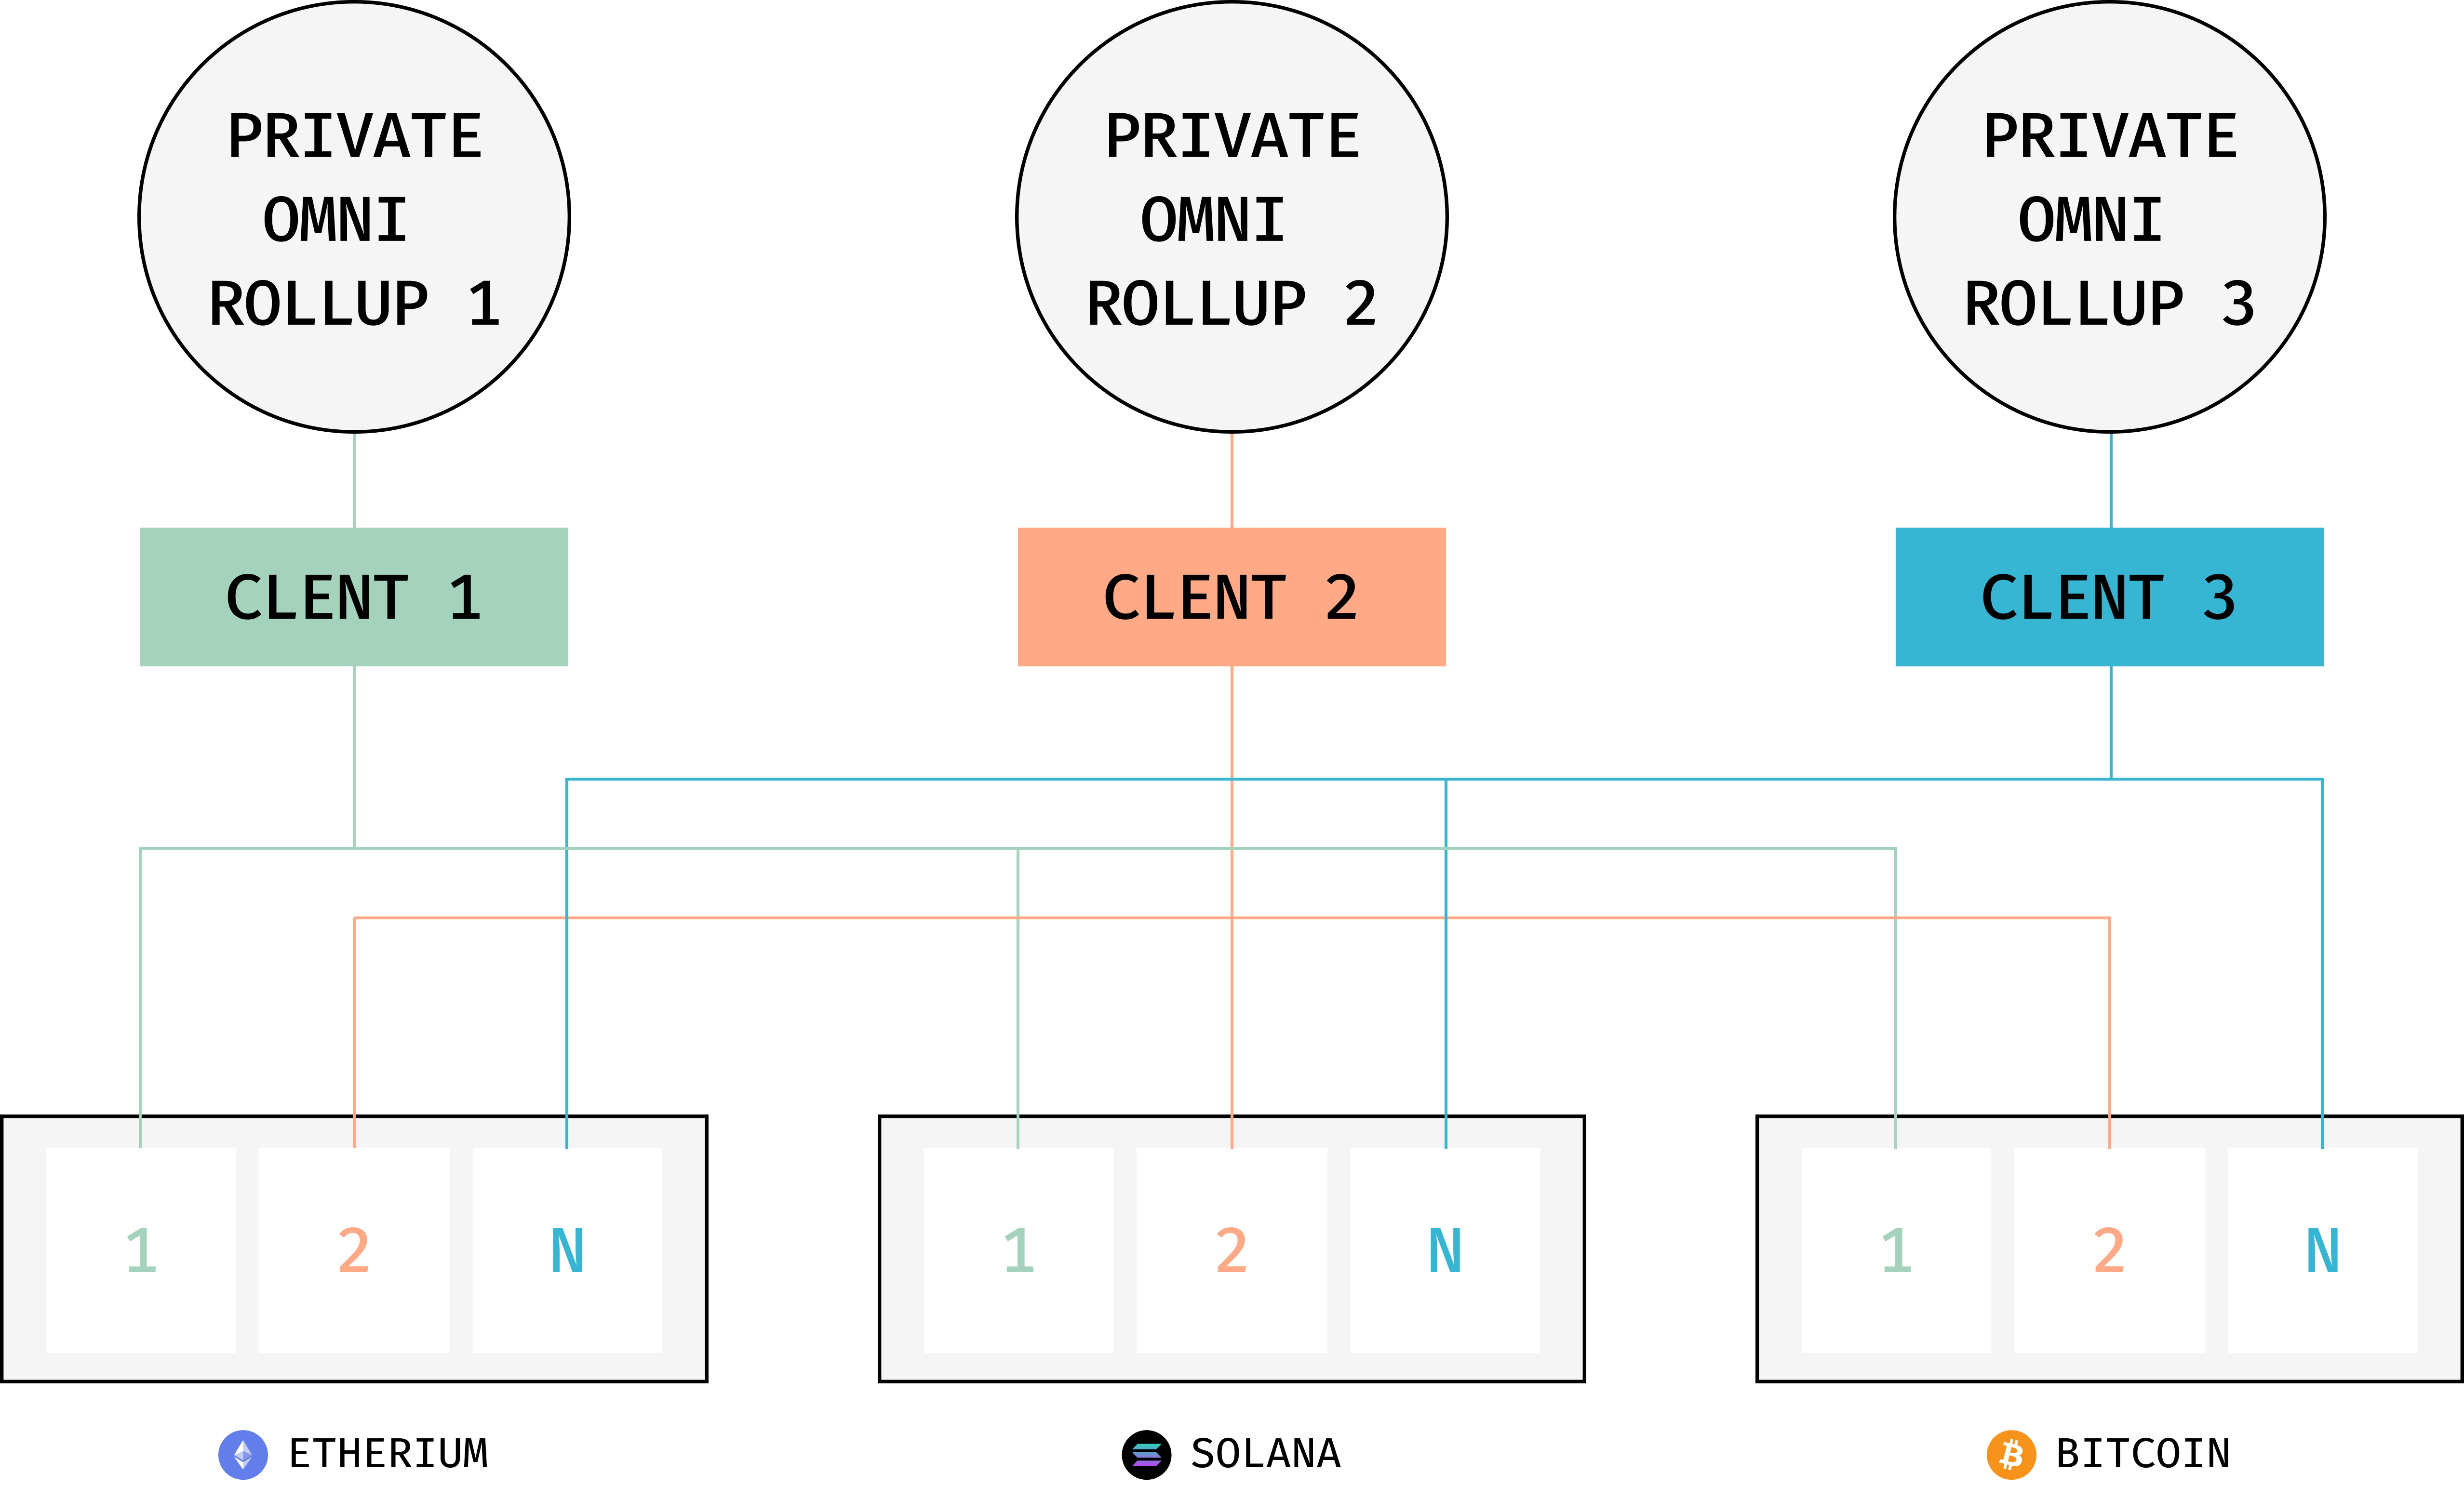
\includegraphics[width=0.9\linewidth]{figure/separate.png}
    \caption{Omni Rollup With Dedicated Executor}
    \label{fig:separate_rollup}
\end{figure}

    \item \textbf{Adapter-Enabled Omni Rollup}  

    This approach builds on existing roll-up infrastructures, transforming them into omni-chain runs through the use of adapters or clients. These adapters facilitate seamless cross-chain communication and functionality without requiring significant modifications to the existing rollup architecture. This method provides a low-barrier entry for projects to integrate into the omnichain ecosystem while preserving their original operational framework. It enables a smooth transition of legacy roll-ups into the omnichain paradigm with minimal disruption.

    \item \textbf{Private Omni Rollup for Enterprise Use}  

    A private omnichain rollup is tailored for enterprise entities to facilitate secure and controlled cross-chain operations. These rollups are maintained by the enterprise itself, with full autonomy over the network execution, consensus, and state management. Designed for privacy and control, they are ideal for corporate applications such as cross-chain payments, supply chain tracking, and private inter-organization workflows. Enterprise solutions requiring controlled, private, and efficient cross-chain infrastructure.  
\end{itemize}

In our omnichain architecture, we are planning to launch a range of omnichain roll-ups, with the potential to scale to tens or even hundreds of thousands. To support this scalability, it is essential that each rollup have secure and decentralized access to its state. This ensures efficient transaction validation and integrity across the entire ecosystem. To achieve this, we collaborated with Linera Microchains. These microchains offer a robust solution by allowing each one to operate independently with its own isolated state. This modularity guarantees that the Omnichain Engine and Sequencer can securely access and validate transactions across all roll-ups, without compromising decentralization or security.

For simpler roll-ups, we will run a Linera node connected to the Ragno Network, providing seamless and straightforward state management. However, for more complex roll-ups with higher liquidity and intricate structures, we will deploy dedicated nodes for each L2/roll-up. This ensures both strong connectivity and thorough verification of transactions. Each microchain will integrate omnichain logic, acting as an intermediary to forward transactions to the sequencer or Hermes, depending on the destination. This setup not only enhances the flexibility and scalability of our solution but also ensures that validation and verification remain fully decentralized, with dedicated validators for each roll-up and microchain.

\subsubsection{Omni Sequencer: The Core of the Omnichain Stack}

The Omni Sequencer is the foundational component of the Omnichain Stack, acting as the central coordination layer for Omni Rollups. It ensures seamless cross-rollup execution, atomic transaction processing, and efficient bundling of transactions across multiple rollup environments. By integrating with both converted L2 rollups (e.g., Optimism, Arbitrum, zkSync, and Movement Labs rollups) and native Omni-rollups, the Omni Sequencer transforms them into fully interoperable Omnichain ecosystems.

 \begin{figure}[h!]
    \centering
    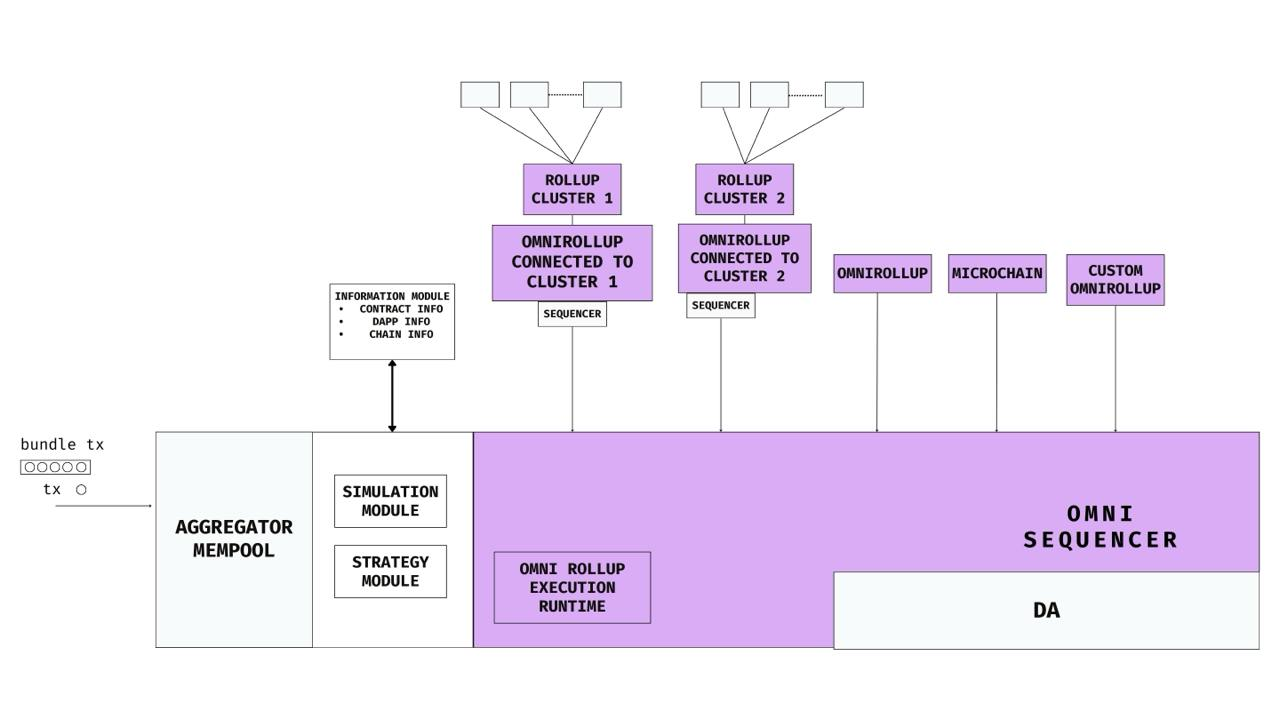
\includegraphics[width=0.99\linewidth]{figure/omnisequencer.jpg}
    \caption{Omnisequencer Overview}
    \label{fig:separate_rollup}
\end{figure}

\textbf{Key Functional Modules of the Omni Sequencer}

\begin{itemize}
    \item[1.] Simulation Module: Ensures atomic execution of transactions across multiple rollups. Simulates transactions before execution to guarantee validity and prevent failures. Reduces transaction reverts by pre-validating state transitions before final submission.

    \item[2.] Strategy Module: Manages transaction ordering and execution logic for cross-rollup transaction bundles. Determines execution priorities based on efficiency, MEV considerations, and state dependencies. Optimizes for low-latency execution and economic efficiency.

    \item[3.] Omni Rollup Execution Runtime: Queries and simulates transaction execution across multiple chains. Facilitates state-aware cross-rollup communication by ensuring each transaction’s dependencies are met. Enhances developer experience by abstracting cross-chain execution complexity.

    \item[4.] Aggregate Mempool: Collects both bundled and individual transactions before execution. Optimizes block space usage by prioritizing transactions based on gas efficiency and finality requirements. Reduces fragmentation in cross-rollup transaction processing.
    
    \item[5.] Data Availability Integration: The Omni Sequencer integrates with multiple DA layers (Data Availability layers) while also maintaining its own Omnichain Data Availability Layer. Enhances data integrity, accessibility, and redundancy across connected rollups. Ensures seamless rollup-to-rollup communication without external dependencies on third-party DA layers.

\end{itemize}
By anchoring the Omnichain Stack, the Omni Sequencer enables true interoperability across rollups. It bridges fragmented L2 ecosystems into a unified execution environment, ensuring that transactions across different chains execute atomically, efficiently, and securely. With its integration of cross-rollup mempools, simulation layers, and DA enhancements, the Omni Sequencer is a game-changer in modular blockchain architecture.

\subsubsection{Transaction Flow and Execution}  
The transaction workflow within the Omni Rollup is a multistage process designed for efficiency, scalability, and cross-chain synchronization. Transactions can originate from various sources, including user submissions, application interactions, or solvers, and are directed to the Omni Sequencer via mempools or other submission mechanisms. Additionally, the sequencer can directly accept transactions initiated on Layer 1 (L1) blockchains through a crawler. The crawler captures and validates these L1 transactions, forwarding them to the Omnichain Engine for direct settlement on the originating L1 chain, bypassing rollups when necessary.  

Once transactions are received, the sequencer organizes them based on predefined criteria such as the target blockchain, the type of operation, or the priority. Within each group, the sequencer determines an optimized execution order to maintain consistency and minimize resource overhead. The ordered transactions are compiled into bundles, with each bundle containing essential metadata, including source and destination chain IDs, timestamps, transaction payloads, and unique nonces to prevent replay attacks.  

To ensure transaction integrity, the Omni Sequencer uses a commitment mechanism. After compiling and ordering the bundles, it generates a cryptographic hash of the ordered transaction list, referred to as the commitment. This hash is published on the Data Availability (DA) Layer, ensuring transparency and allowing participants to validate the accuracy of the transaction order by comparing the commitment with the actual processing sequence during execution.  

The sequencer then distributes the bundled transactions to the appropriate rollups for execution. Each rollup begins by verifying the transaction order against the commitment published on the DA layer, ensuring alignment with the global sequence determined by the sequencer. Transactions are processed in accordance with this verified order, and the rollup computes state transitions for the respective blockchain or application.  

To guarantee security and integrity, the rollup uses zero-knowledge (zk) proofs generated by the Prover Network. These zk proofs validate the correctness of state transitions without exposing sensitive data, ensuring that the process is both tamperproof and privacy-preserving. For contract-enabled blockchains, rollups interact directly with smart contracts to manage state updates, validate proofs, and finalize transactions on the L1 chain. For blockchains without smart contract support, the rollup uses direct addresses, also known as vaults, as custodial points for assets and data. These vaults ensure that transactions and state updates are accurately reflected despite the lack of native contract capabilities.  

In both cases, rollups send the updated states and zk proofs to the respective L1 chains for inclusion in their blocks. This ensures that state changes are synchronized across the network, maintaining consistency across all connected chains. By supporting both direct L1 transactions and rollup-based processing, Omni Rollup establishes a robust, scalable, and trustless framework for cross-chain transactions, enhancing interoperability, and ensuring data integrity across diverse blockchain ecosystems.  

\subsubsection{Transaction Conflict Resolution}
The Omni Sequencer employs a robust mechanism to detect and resolve transaction conflicts, ensuring consistency and preventing double spending on multiple rollups. To achieve this, the sequencer maintains a global transaction pool, aggregating all incoming transactions, including those targeting different rollups. Before determining the execution order, the sequencer analyzes the input dependencies of each transaction (for example, the user's ETH balance). If multiple transactions reference the same input, a dependency conflict is detected.

In such cases, the sequencer assigns a global execution order to all transactions. Among conflicting transactions (e.g., double-spend attempts), only the first valid transaction in the sequence is included for execution, while subsequent conflicting transactions are marked as invalid or rejected outright. The ordered transactions, along with a cryptographic commitment to their order, are published on the Data Availability (DA) layer, ensuring transparency and verifiability. The sequencer then distributes the bundled transactions to their respective rollups for execution.

Each rollup verifies the transaction order against the published commitment. Transactions flagged as invalid or rejected by the sequencer are excluded during execution. This ensures that only valid transactions progress to state updates, maintaining the integrity and consistency of operations across all rollups in the Omnichain ecosystem.